\documentclass[10pt]{article}
\usepackage[margin=0.78in]{geometry}
\usepackage[T1]{fontenc}
\usepackage{lmodern}
\usepackage{microtype}
\usepackage{amsmath,amssymb,booktabs,array}
\usepackage{graphicx,xcolor,tikz,listings}
\usetikzlibrary{arrows.meta,positioning,fit,calc}
\usepackage[colorlinks=true,linkcolor=blue!45!black,urlcolor=blue!45!black,citecolor=blue!45!black]{hyperref}
\definecolor{memorygreen}{RGB}{29,105,83}
\definecolor{controlblue}{RGB}{42,85,132}
\definecolor{evidencered}{RGB}{155,58,64}
\lstset{basicstyle=\ttfamily\footnotesize,breaklines=true,columns=fullflexible,keepspaces=true,frame=single,rulecolor=\color{black!15},backgroundcolor=\color{black!2},xleftmargin=5pt,xrightmargin=5pt,aboveskip=8pt,belowskip=8pt}
\setlength{\parindent}{0pt}
\setlength{\parskip}{5pt}
\setlength{\emergencystretch}{2em}
\newcommand{\module}[1]{\textcolor{controlblue}{\textbf{#1}}}
\title{Discovering What a Robot Must Remember for Safety}
\author{}
\date{}
\begin{document}
\maketitle
\vspace{-2.5em}
\begin{abstract}
We propose a persistent safety-memory architecture for vision-language-action (VLA) policies. The central hypothesis is that safety experience should teach a robot to discover new history-dependent state variables, retain their update mechanisms across deployments, and use them to evaluate proposed actions. The design separates episode beliefs, persistent mechanisms, and immutable evidence. This document specifies the system pipeline, interfaces, learning loop, and a complete numerical example. It is a research proposal: the accompanying executable replay validates the example's memory and action-selection arithmetic, not perception, autonomous mechanism discovery, or physical robot safety.
\end{abstract}

\section{Main System Design}
The system receives camera images $I_t$, proprioception $q_t$, an instruction $\ell$, and previous actions. A nominal VLA proposes an action chunk. In parallel, tracked events update object-bound safety beliefs using previously learned mechanisms. Retrieval is conditioned on the proposed interaction, not only image or instruction similarity. A risk evaluator then selects an acceptable action or recovery plan. Experience is stored for slower refinement of the memory representation.

\begin{figure}[h!]
\centering
\resizebox{\linewidth}{!}{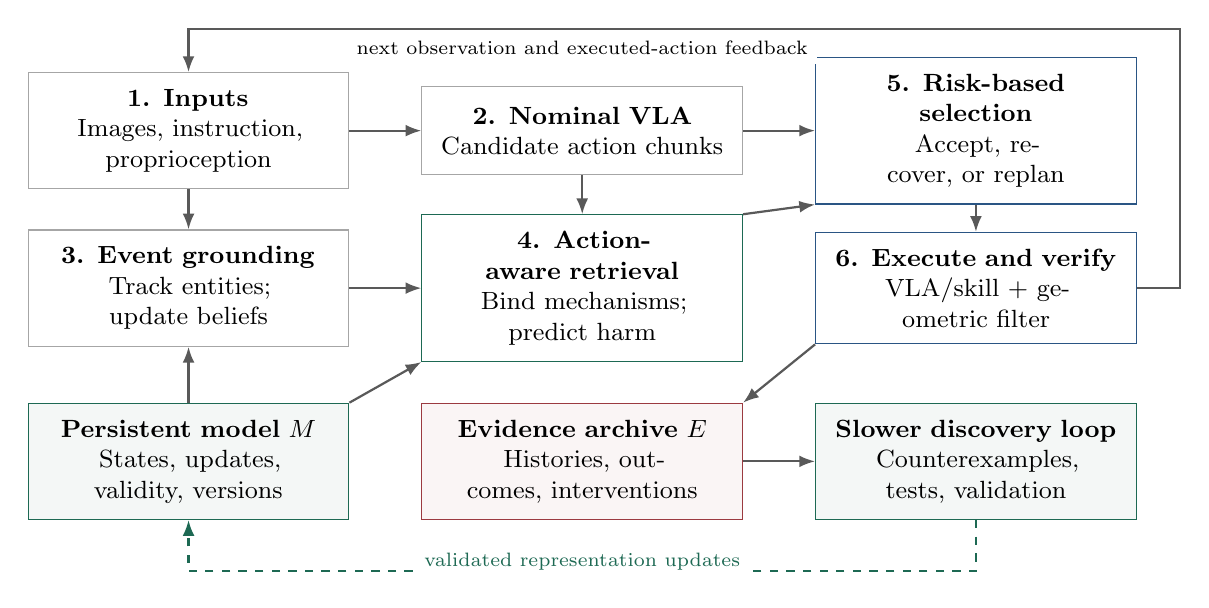
\begin{tikzpicture}[
  box/.style={draw=black!35,fill=white,align=center,text width=3.65cm,minimum height=1.12cm,inner sep=6pt,font=\small},
  flow/.style={-{Latex[length=2mm]},thick,draw=black!65},
  slow/.style={flow,dashed,draw=memorygreen}]
\node[box] (input) at (0,0) {\textbf{1. Inputs}\\Images, instruction, proprioception};
\node[box] (vla) at (5,0) {\textbf{2. Nominal VLA}\\Candidate action chunks};
\node[box,draw=controlblue] (select) at (10,0) {\textbf{5. Risk-based selection}\\Accept, recover, or replan};
\node[box] (events) at (0,-2) {\textbf{3. Event grounding}\\Track entities; update beliefs};
\node[box,draw=memorygreen] (retrieve) at (5,-2) {\textbf{4. Action-aware retrieval}\\Bind mechanisms; predict harm};
\node[box,draw=controlblue] (execute) at (10,-2) {\textbf{6. Execute and verify}\\VLA/skill + geometric filter};
\node[box,draw=memorygreen,fill=memorygreen!5] (model) at (0,-4.2) {\textbf{Persistent model $M$}\\States, updates, validity, versions};
\node[box,draw=evidencered,fill=evidencered!5] (archive) at (5,-4.2) {\textbf{Evidence archive $E$}\\Histories, outcomes, interventions};
\node[box,draw=memorygreen,fill=memorygreen!5] (learn) at (10,-4.2) {\textbf{Slower discovery loop}\\Counterexamples, tests, validation};
\draw[flow] (input)--(vla);
\draw[flow] (vla)--(select);
\draw[flow] (input)--(events);
\draw[flow] (events)--(retrieve);
\draw[flow] (vla)--(retrieve);
\draw[flow] (retrieve.north east)--(select.south west);
\draw[flow] (select)--(execute);
\draw[flow] (model)--(events);
\draw[flow] (model.north east)--(retrieve.south west);
\draw[flow] (execute.south west)--(archive.north east);
\draw[flow] (archive)--(learn);
\draw[slow] (learn.south)--++(0,-0.65)-|(model.south);
\node[font=\scriptsize,text=memorygreen,fill=white] at (5,-5.48) {validated representation updates};
\draw[flow] (execute.east)--++(0.55,0)|-($(input.north)+(0,0.55)$)--(input.north);
\node[font=\scriptsize,fill=white] at (5,1.05) {next observation and executed-action feedback};
\end{tikzpicture}
}
\caption{Two-timescale architecture. Solid arrows carry online decisions and evidence. Dashed arrows carry slower validated model updates. The VLA proposes; memory changes which proposals are accepted and which recovery subgoals are issued. All modules beyond the base policy are proposed components.}
\label{fig:pipeline}
\end{figure}

\textbf{Research contribution.} Learn a missing safety state and its executable temporal update mechanism from discrepant outcomes, then reuse it across objects and tasks. Storing warnings, retrieving failure episodes, and adding a geometric safety filter are supporting components, not sufficient novelty claims.

\newpage
\section{Memory: What Is Stored and What Changes}
\subsection{Three distinct stores}
\begin{center}
\small
\begin{tabular}{p{0.18\linewidth}p{0.40\linewidth}p{0.32\linewidth}}
\toprule
Store & Contents & Lifetime and use \\
\midrule
Episode belief $z_t$ & Object IDs, latent-state probabilities, relevant event references, tracking uncertainty & Updated every observation; reset only when physical reset is justified. \\
Persistent model $M$ & Typed state definitions, event-conditioned transitions, hazard predictors, applicability, versions & Survives deployments; instantiated on new objects by role. \\
Evidence archive $E$ & Images, actions proposed/executed, outcomes, interventions, provenance, diagnostic pairs & Append-only source of evidence for discovery, correction, and regression tests. \\
\bottomrule
\end{tabular}
\end{center}

\subsection{Executable mechanism representation}
A mechanism is a tuple
\[
m=(\mathcal R,\mathcal Z,f_{\rm obs},f_{\rm update},g_{\rm harm},\mathcal D,E^+,E^-,E^?,v),
\]
where $\mathcal R$ contains typed argument roles; $\mathcal Z$ is a Boolean, categorical, or continuous latent-state domain; $f_{\rm obs}$ grounds observations; $f_{\rm update}$ updates beliefs; $g_{\rm harm}$ predicts action-dependent risk; and $\mathcal D$ specifies validity limits and diagnostic tests. Evidence distinguishes support, contradiction, and unresolved/censored outcomes. A name such as \texttt{exposed} is an interpretation, not proof that the state is correctly grounded.

\textbf{Why hybrid memory?} Logic provides relational binding and explicit temporal structure. Probabilities represent uncertain perception and transitions. Continuous state supports quantities such as temperature or accumulated load. Embeddings help retrieve candidate evidence but do not establish that a mechanism applies.

\subsection{Storage and retrieval interfaces}
Use structured tables for mechanisms, bindings, versions, and evidence metadata; an object store for clips and sensor traces; and an embedding index for approximate evidence search. A graph or indexed relation table records dependencies between contacts, entities, and latent states. The particular database is an engineering choice, not the research contribution.

\begin{lstlisting}
update_belief(images, proprioception, last_action, z, M) -> z_next
propose_vla(images, instruction, proprioception) -> action_chunks
retrieve(z_next, action_chunks, M) -> bound_mechanisms, evidence_ids
evaluate(action_chunks, z_next, bound_mechanisms) -> risks, uncertainty
select_or_recover(action_chunks, risks, instruction) -> executable_plan
append_evidence(proposed, executed, observation, outcome, provenance)
refine_offline(E, M) -> candidate_model -> regression_gate -> M_next
\end{lstlisting}

For each chunk, infer candidate contacts and interaction roles. Retrieve mechanisms connected to those roles, then follow their evidence dependencies. Always evaluate applicable known hard monitors; do not discard them because they fall outside a vector-search top-$k$. An unresolved object identity or unsupported mechanism binding should trigger uncertainty handling.

\newpage
\section{How Safety Knowledge Accumulates}
\subsection{Discovering a missing state}
Suppose two histories map to the same current representation, yet the same future intervention produces different safety-outcome distributions. This is evidence of possible state aliasing. One differing outcome is insufficient under noise. Repeated trials or a calibrated discrepancy test must separate a missing variable from stochasticity, model error, and incorrect tracking.

The learner proposes refinements from a declared grammar: persistence, reset, time decay, bounded counting, and relational propagation. Neural detectors ground events; small recurrent programs or automata retain their effects. A VLM may suggest hypotheses, but held-out interventions select among them. The system does not claim to invent arbitrary physics from pixels.

\begin{enumerate}
\item Record histories with outcome discrepancies under comparable actions.
\item Retrieve earlier events that could explain the discrepancy.
\item Propose competing state/update programs, including a no-refinement hypothesis.
\item Query valid simulator branches or verified feedback that distinguish candidates.
\item Fit candidates using outcome prediction, complexity, and past-hazard regression losses.
\item Promote a validated version; retain counterexamples and uncertain alternatives.
\end{enumerate}

\subsection{Example discovery sequence}
\begin{center}
\small
\begin{tabular}{p{0.15\linewidth}p{0.38\linewidth}p{0.36\linewidth}}
\toprule
Stage & Evidence & Change to persistent memory \\
\midrule
$M_0$ & Current geometry cannot explain different outcomes after earlier contact. & No exposure state; report unresolved risk. \\
Candidate & Contact/no-contact branches differ despite matching final scenes. & Propose persistent object-bound exposure state. \\
$M_1$ & Held-out contacts reproduce transfer across different objects. & Retain contact-triggered update and action-risk predictor. \\
$M_2$ & Verified cleaning lowers risk; ineffective cleaning does not. & Add conditional reset, efficacy uncertainty, and negative evidence. \\
Transfer & A new tool participates in a longer contact chain. & Rebind and compose existing mechanism; revise only if evidence requires it. \\
\bottomrule
\end{tabular}
\end{center}

\textbf{Selective feedback.} A blocked nominal action has an unknown counterfactual outcome. A safe replacement does not validate the rejected action. Store \texttt{counterfactual\_outcome: unknown}, with any simulator or assessor estimates labeled separately.

\textbf{Scientific boundary.} Predictive state, safety-aware representation learning, predicate invention, and counterexample refinement already exist~\cite{psr,fusion,interpret,predicate,cegar}. SOMA already combines contrastive memory with VLA orchestration~\cite{soma}; EventVLA learns event-oriented visual memory~\cite{eventvla}. The candidate contribution is their specific unresolved intersection: continual invention of history-dependent safety state, validated through interventions and transferred compositionally into VLA control. Priority is not established merely by combining these terms.

\newpage
\section{Worked Example: Images and Instruction}
\textbf{Task instruction:} ``Use the tool to move the white block into the green tray.''

\textbf{Observation stream:} RGB frames show a tool contacting a marked source, moving away, and later approaching the block. The current image alone does not reveal the previous contact. The source marker is a simulated exposure cue, not a claim that real contamination is visually observable.

\begin{figure}[h!]
\centering
\resizebox{\linewidth}{!}{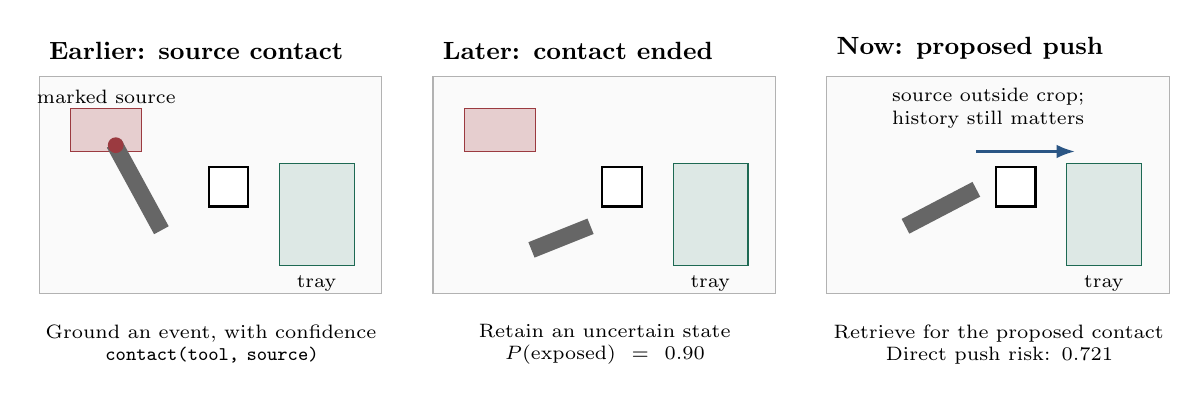
\begin{tikzpicture}[font=\small]
\foreach \x/\label in {0/{Earlier: source contact},5/{Later: contact ended},10/{Now: proposed push}} {
  \draw[fill=black!2,draw=black!30] (\x,0) rectangle ++(4.35,2.75);
  \node[anchor=south west,font=\small\bfseries] at (\x,2.85) {\label};
  \draw[fill=memorygreen!15,draw=memorygreen] (\x+3.05,0.35) rectangle ++(0.95,1.3);
  \node[font=\scriptsize] at (\x+3.52,0.12) {tray};
  \draw[fill=white,thick] (\x+2.15,1.1) rectangle ++(0.5,0.5);
}
\draw[fill=evidencered!25,draw=evidencered] (0.4,1.8) rectangle ++(0.9,0.55);
\node[font=\scriptsize] at (0.85,2.5) {marked source};
\draw[line width=6pt,draw=black!60] (0.95,1.9)--(1.55,0.8);
\fill[evidencered] (0.97,1.88) circle (0.1);
\draw[fill=evidencered!25,draw=evidencered] (5.4,1.8) rectangle ++(0.9,0.55);
\draw[line width=6pt,draw=black!60] (6.25,0.55)--(7,0.85);
\draw[line width=6pt,draw=black!60] (11,0.85)--(11.9,1.32);
\draw[-{Latex},thick,draw=controlblue] (11.9,1.8)--(13.15,1.8);
\node[font=\scriptsize,align=center] at (12.05,2.35) {source outside crop;\\history still matters};
\node[align=center,text width=4.2cm,font=\scriptsize] at (2.18,-0.65) {Ground an event, with confidence\\\texttt{contact(tool, source)}};
\node[align=center,text width=4.2cm,font=\scriptsize] at (7.18,-0.65) {Retain an uncertain state\\$P(\mathrm{exposed})=0.90$};
\node[align=center,text width=4.2cm,font=\scriptsize] at (12.18,-0.65) {Retrieve for the proposed contact\\Direct push risk: $0.721$};
\end{tikzpicture}
}
\caption{Schematic camera inputs, not robot recordings. The source is visible in the earlier frame but outside the current crop. An alternative history with no prior source contact has the same current frame and a different safe decision.}
\label{fig:frames}
\end{figure}

\subsection{Step 1: Perception updates episode memory}
An object tracker identifies \texttt{tool\_7}, \texttt{source\_2}, \texttt{block\_4}, and \texttt{tray\_1}. Event grounding produces \texttt{contact(tool\_7, source\_2)}. The already validated mechanism $M_2$ updates the exposure belief to $P(e_{\texttt{tool\_7}}=1)=0.90$. This value is stipulated for the numerical example; a real system must infer and calibrate it from sensing and transition evidence.

\subsection{Step 2: The nominal VLA proposes contact}
The base policy proposes a chunk that approaches the block and begins pushing it. A chunk interaction predictor maps the continuous trajectory to the candidate relation \texttt{contact(tool\_7, block\_4)}. This mapping is a required learned or geometric component, not a capability assumed to emerge from text retrieval.

\subsection{Step 3: Retrieval binds the relevant mechanism}
The query contains the actor role \texttt{tool\_7}, receiver \texttt{block\_4}, proposed contact, current exposure belief, and task intent. It retrieves \texttt{contact\_transfer@v2}, the earlier source-contact event, and the validated reset mechanism. The relevant experience could involve a visually different tool; relational role compatibility is more important than image similarity.

\subsection{Step 4: Risk changes the decision}
The illustrative mechanism gives harmful transfer probability $0.80$ when the tool is exposed and $0.01$ otherwise. Thus direct contact has risk
\[
r_{\rm direct}=0.90(0.80)+0.10(0.01)=0.721.
\]
At an illustrative acceptance threshold $\tau=0.05$, this proposal is rejected. The number is a toy decision threshold, not a certified physical safety tolerance. The next page shows the exact memory that supports this decision.

\newpage
\section{Concrete Memory Records}
\textbf{Persistent mechanism:} executable structure shared across episodes. Numbers below are illustrative and intentionally match the runnable replay.
\begin{lstlisting}
id: contact_transfer
version: 2
roles: {actor: tracked_tool, receiver: protected_object}
state: {name: exposure, domain: Bernoulli_belief}
activation: proposed_contact(actor, receiver)
update:
  source_contact: infer_exposure_from_event_and_source_belief
  no_relevant_event: persist
  validated_cleaning: p_exposure *= 0.03
risk:
  harm_given_exposed: 0.80
  harm_given_unexposed: 0.01
scope: simulated_marker_transfer; validated_tool_materials
evidence:
  support: [branch_12, branch_19, reset_trial_8]
  contradiction: [ineffective_cleaning_trial_3]
  unresolved: [blocked_contact_41]
status: illustrative_validated_model
\end{lstlisting}

\textbf{Episode state:} the mechanism instantiated on the currently tracked tool.
\begin{lstlisting}
episode: 42
entity: tool_7
belief: {exposure: 0.90}
last_relevant_event: contact_17
event_evidence: {frame_ids: [I_17, I_18], source: source_2}
mechanism: contact_transfer@v2
retrieval_query:
  proposed_event: contact(tool_7, block_4)
  instruction_intent: move(block_4, tray_1)
\end{lstlisting}

\textbf{Intervention record:} nominal actions and actual outcomes remain separate.
\begin{lstlisting}
decision: blocked_contact_41
proposed: push(tool_7, block_4)
predicted_risk: 0.721
executed_instead: clean_verify_then_push(tool_7, block_4)
counterfactual_outcome_of_proposed: unknown
executed_outcome: {task_complete: true, marker_transfer: false}
outcome_source: illustrative_simulator_feedback
update_target: recovery_evidence_only
\end{lstlisting}
The last record does not imply that a single successful recovery proves the mechanism. New evidence is appended; mechanism parameters and structure change only through the separate validation loop.

\newpage
\section{From Memory to VLA Actions}
\subsection{Candidate plans and selection}
Suppose a previously validated cleaning skill leaves exposure probability $0.90\times0.03=0.027$, while a verified replacement tool has exposure probability $0.01$. Assume, only for this toy calculation, that transit and cleaning introduce no additional hazards. A deployed evaluator must include risks throughout each recovery plan and the subsequent task, not only endpoint contact.

\begin{center}
\begin{tabular}{lrrl}
\toprule
Candidate plan & Predicted risk & Effort cost & Decision at $\tau=0.05$ \\
\midrule
Direct push & $0.72100$ & 0 & Reject \\
Wait, then push & $0.72100$ & 0.5 & Reject: exposure persists \\
Clean, verify, then push & $0.03133$ & 1 & Accept; least-cost acceptable \\
Use verified replacement & $0.01790$ & 2 & Accept; higher effort \\
\bottomrule
\end{tabular}
\end{center}

The generic selector is
\[
a^* = \arg\min_{a\in\mathcal A_t} C_{\rm task}(a)+\lambda C_{\rm deviation}(a)
\quad\text{subject to}\quad \overline r(a\mid z_t,M)\leq\tau,
\]
where $\overline r$ should account for model and belief uncertainty. The replay uses point estimates solely to make the arithmetic transparent. Calibration and out-of-distribution handling remain research requirements.

\subsection{The actual interface to the VLA}
The controller initially withholds the push chunk. A subgoal manager sends ``Move the tool to the cleaning station and execute the validated cleaning skill'' to the appropriate skill executor. If the VLA cannot reliably execute that skill, use a validated controller or decline that candidate. After execution, verification updates the belief; merely issuing the instruction does not reset the state.

Once verification succeeds, the system asks the VLA to resume the original block-moving instruction. It rescores the new chunk using the updated belief, then executes through the geometric safety layer. If verification fails or is unavailable, retain uncertainty and replan; do not assume cleaning worked.

This creates an explicit chain:
\[
\text{memory belief}\rightarrow\text{action risk}\rightarrow\text{chunk withheld}
\rightarrow\text{recovery subgoal}\rightarrow\text{verified update}\rightarrow\text{VLA resumes}.
\]
An optional later extension can inject memory tokens or risk gradients into action generation. The initial design uses selection and recovery because these expose exactly how memory alters behavior. A geometric CBF remains useful for motion hazards but does not enforce the exposure mechanism by itself.

\subsection{Executable replay and comparison}
Run \texttt{python3 example\_replay.py}. The script asserts the table values, the selected recovery, retention of the belief after failed verification, and the opposite decision for a visually identical clean-history case. Its mechanisms and beliefs are supplied, not learned. It is a deterministic interface test and worked example, not an implemented VLA or a demonstration of state invention.

\newpage
\section{Research Validation and Scope}
\textbf{Decisive experiment.} Start without the exposure state, learn it from matched-history intervention evidence, then test new objects and longer transfer chains. Compare against full-history recurrent memory, event retrieval, fixed-vocabulary rules, and an oracle state model. Match observations, feedback, simulator query budget, VLA, and recovery access. A larger memory or additional privileged feedback must not explain the gain.

\textbf{Accumulation metrics.} Measure repeat-hazard rate versus deployment experience, safe task completion, unnecessary interventions, retention on previous mechanisms, held-out compositional transfer, risk calibration, and latency. Evaluate harm with an independent simulator scorer, not the learned memory's own labels.

\textbf{Failure conditions.} Missing history may be unidentifiable; perception may bind an event to the wrong object; simulator counterfactuals may be invalid; representation growth may overfit; a world change may invalidate an old mechanism. Preserve uncertainty and provenance. Claims of formal safety require explicit assumptions beyond this proposal.

\textbf{Implementation order.} First build the evidence/belief/selection interfaces and paired-history simulator test. Next implement one bounded state-invention grammar and diagnostic interventions. Only then connect the learned model to a full VLA and broaden the hazard families. The existing SafeLIBERO-style motion filter can remain the low-level component, but history-dependent hazards require additional instrumentation.

\begin{thebibliography}{9}
\small
\bibitem{psr} M. L. Littman, R. S. Sutton, and S. Singh. \emph{Predictive Representations of State}. NeurIPS, 2001. \href{https://proceedings.neurips.cc/paper/2001/file/1e4d36177d71bbb3558e43af9577d70e-Paper.pdf}{Primary paper}.
\bibitem{fusion} H. Lin et al. \emph{Safety-aware Causal Representation for Trustworthy Offline Reinforcement Learning in Autonomous Driving}. RA-L, 2024. \href{https://hhlin.info/publication/fusion/}{Author publication page}.
\bibitem{interpret} \emph{InterPreT: Interactive Predicate Learning from Language Feedback for Generalizable Task Planning}. RSS, 2024. \href{https://www.roboticsproceedings.org/rss20/p034.pdf}{Proceedings paper}.
\bibitem{predicate} \emph{Predicate Invention for Bilevel Planning}. AAAI, 2023. \href{https://ojs.aaai.org/index.php/AAAI/article/view/26429}{Publisher paper}.
\bibitem{cegar} \emph{Counterexample-guided Abstraction Refinement for POMDPs}. Preprint, 2017. \href{https://arxiv.org/abs/1701.06209}{arXiv:1701.06209}.
\bibitem{soma} Z. Li, Z. Li, K. Zhou, and J. Gu. \emph{SOMA: Strategic Orchestration and Memory-Augmented System for Vision-Language-Action Model Robustness via In-Context Adaptation}. Preprint, March 2026. \href{https://arxiv.org/abs/2603.24060}{arXiv:2603.24060}.
\bibitem{eventvla} G. Yang et al. \emph{EventVLA: Event-Driven Visual Evidence Memory for Long-Horizon Vision-Language-Action Policies}. Preprint, June 2026. \href{https://arxiv.org/abs/2606.20092}{arXiv:2606.20092}.
\end{thebibliography}

\textit{Evidence scope:} This is a design document, not an exhaustive literature survey. The companion Markdown reports provide a broader source map, including SkillWrapper, VisualPredicator, safe predictive-state learning, constraint learning, and existing VLA safety guidance. Source maturity varies; no numerical comparison with published systems is claimed here.
\end{document}
